% =====================================================================
\section{Kết quả thực nghiệm}
\label{sec:results}
% =====================================================================

Trong phần này, mọi giá trị số đều được đọc trực tiếp từ các tệp
\code{results/checkpoints/*.json} do quá trình huấn luyện sinh ra. Không có giá trị nào được
nhập bằng tay.

\subsection{Khối thực nghiệm chính}
\label{sec:results-main}

Khối thực nghiệm hoàn thành \RRuns{} lượt huấn luyện ($3$ cấu hình $\times$ $3$ mức nhãn
$\times$ $3$ lần lặp), tổng thời gian huấn luyện \RTotalHours{} giờ trên
\REnvGpu{}. Chi tiết từng lượt được liệt kê ở \tabref{tab:per-run}; bảng tổng hợp kết quả trên
tập test là \tabref{tab:main-results}.

% Sinh tự động — scripts/make_report_data.py
\begin{table}[htbp]
  \centering
  \scriptsize
  \setlength{\tabcolsep}{4.5pt}
  \begin{tabular}{@{}l r r r r r r r r r@{}}
    \toprule
    \multirow{2}{*}{\makecell[l]{Cấu hình}} & \multicolumn{3}{c}{10\,\% nhãn} & \multicolumn{3}{c}{20\,\% nhãn} & \multicolumn{3}{c}{50\,\% nhãn} \\
    \cmidrule(lr){2-4}\cmidrule(lr){5-7}\cmidrule(lr){8-10}
     & Macro-F1 & Acc. & $\Delta$ & Macro-F1 & Acc. & $\Delta$ & Macro-F1 & Acc. & $\Delta$ \\

    \midrule
    \cfg{E1} & 0,9319 & 0,9349 & --- & 0,9497 & 0,9517 & --- & 0,9690 & 0,9702 & --- \\
    \cfg{E2-L} & 0,9313 & 0,9340 & $$-$0,06$ & 0,9505 & 0,9524 & $+0,08$ & 0,9745 & 0,9755 & $+0,55$ \\
    \cfg{E2} & 0,9470 & 0,9492 & $+1,51$ & 0,9631 & 0,9645 & $+1,34$ & 0,9777 & 0,9786 & $+0,88$ \\
    \bottomrule
  \end{tabular}
  \caption{Kết quả trên $\Dtest$: Macro-F1 và Accuracy (\enquote{Acc.}) là trung bình qua ba lần lặp. $\Delta$ là chênh lệch Macro-F1 trung bình so với \cfg{E1} ở cùng mức nhãn, tính bằng điểm phần trăm; giá trị dương nghĩa là cấu hình đa nhiệm tốt hơn baseline. Độ lệch chuẩn qua ba lần lặp được báo cáo ở \tabref{tab:main-std}.}
  \label{tab:main-results}
\end{table}

% Sinh tự động — scripts/make_report_data.py
\begin{table}[htbp]
  \centering
  \small
  \setlength{\tabcolsep}{5pt}
  \begin{tabular}{@{}l c c c@{}}
    \toprule
    Cấu hình & 10\,\% nhãn & 20\,\% nhãn & 50\,\% nhãn \\
    \midrule
    \cfg{E1} & $0,9319 \pm 0,0035$ & $0,9497 \pm 0,0030$ & $0,9690 \pm 0,0015$ \\
    \cfg{E2-L} & $0,9313 \pm 0,0030$ & $0,9505 \pm 0,0027$ & $0,9745 \pm 0,0017$ \\
    \cfg{E2} & $0,9470 \pm 0,0034$ & $0,9631 \pm 0,0047$ & $0,9777 \pm 0,0022$ \\
    \bottomrule
  \end{tabular}
  \caption{Macro-F1 trên $\Dtest$ dạng trung bình $\pm$ độ lệch chuẩn mẫu qua ba lần lặp. Ba lần lặp chỉ cung cấp bằng chứng ban đầu về độ ổn định, không đủ để kết luận về ý nghĩa thống kê.}
  \label{tab:main-std}
\end{table}

\begin{figure}[htbp]
  \centering
  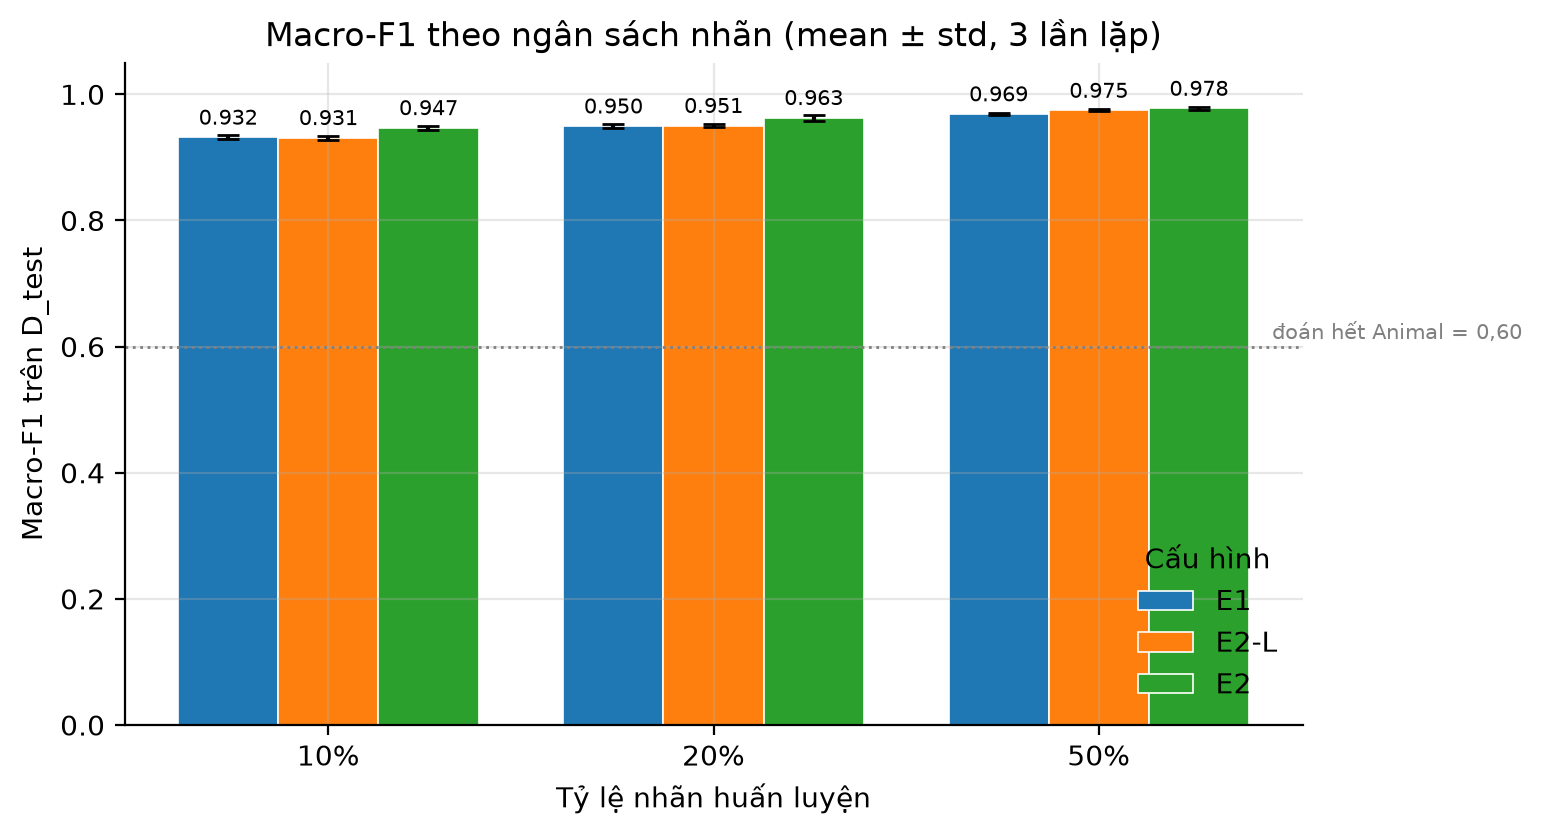
\includegraphics[width=\textwidth]{../results/figures/fig02_macro_f1_by_budget.png}
  \caption{Macro-F1 trên $\Dtest$ theo ngân sách nhãn cho ba cấu hình. Cột là trung bình qua ba
  lần lặp, thanh sai số là một độ lệch chuẩn mẫu. Đường chấm ngang ở $0{,}60$ đánh dấu mức
  Accuracy của bộ phân loại luôn đoán \enquote{Animal}; mọi cấu hình đều vượt mức này rõ rệt.}
  \label{fig:macro-f1}
\end{figure}

\begin{figure}[htbp]
  \centering
  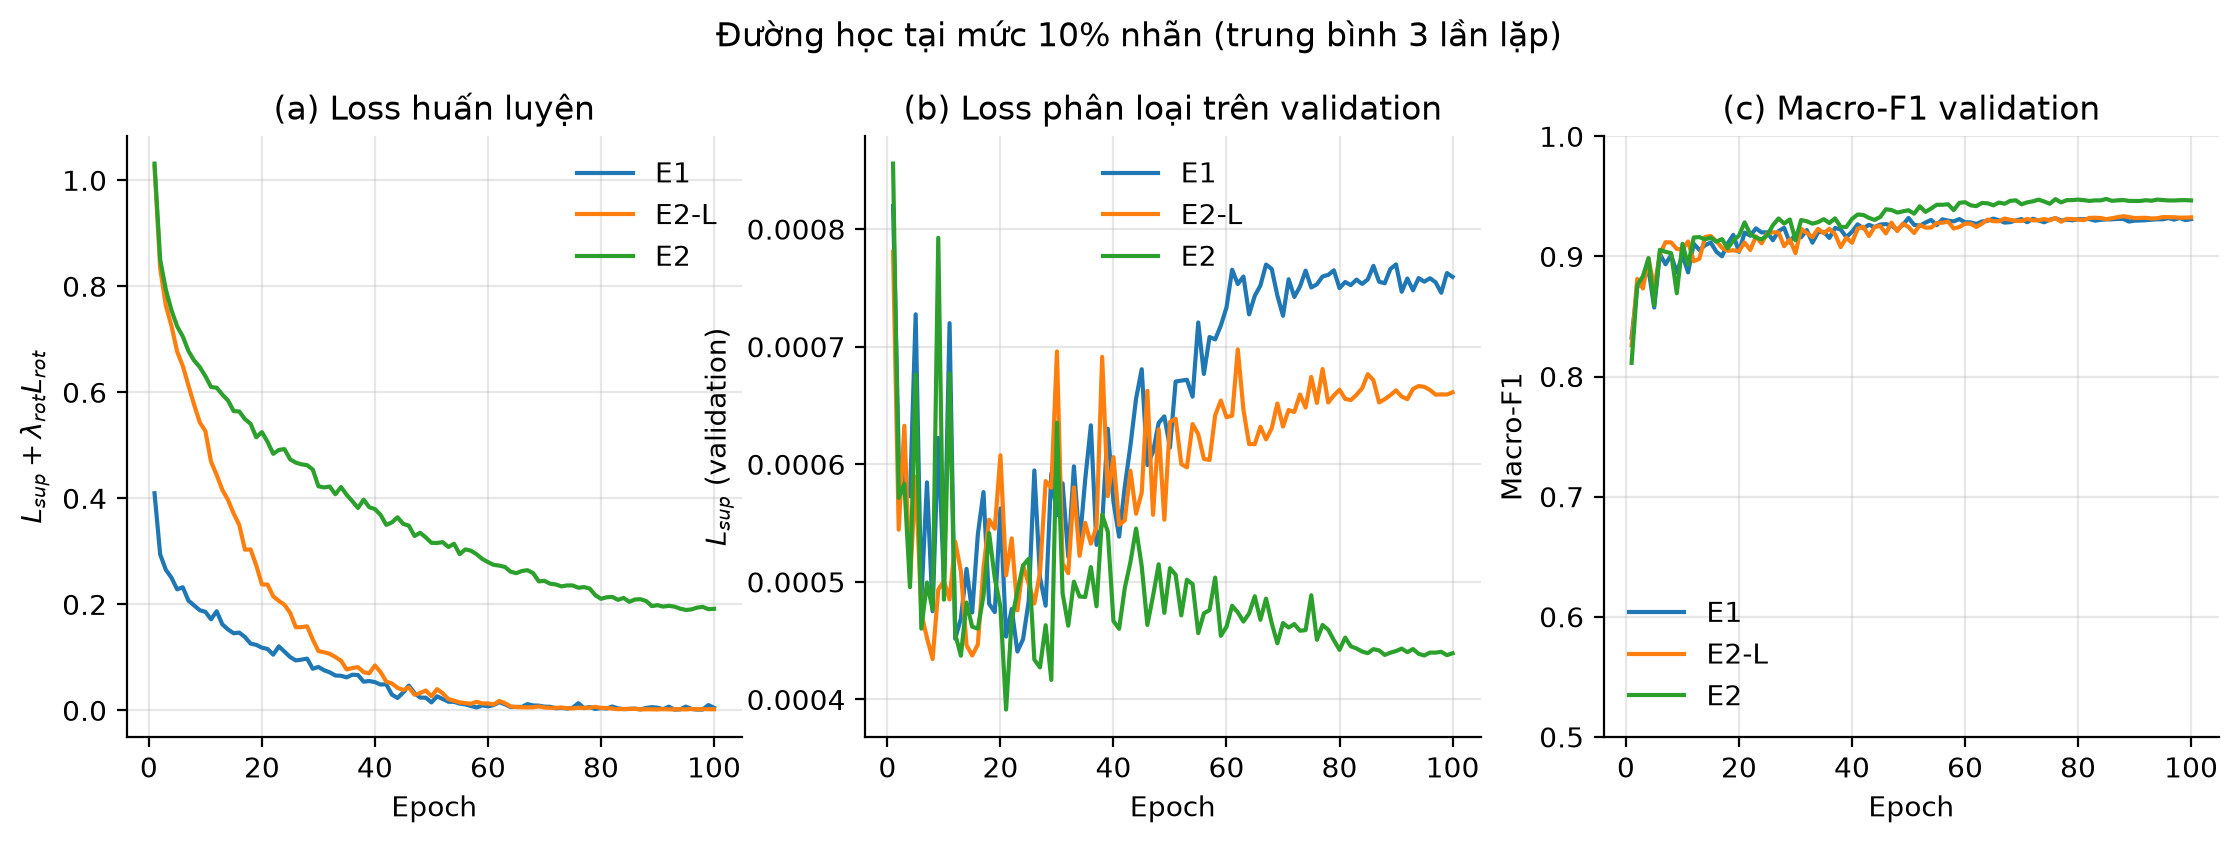
\includegraphics[width=\textwidth]{../results/figures/fig01_learning_curves_L10.png}
  \caption{Đường học tại mức $10\,\%$ nhãn, trung bình qua ba lần lặp. (a)~Loss huấn luyện
  gồm cả hai nhánh; (b)~loss phân loại trên validation; (c)~Macro-F1 validation. Ở cấu hình
  \cfg{E1} nhánh phụ không tồn tại nên $L_{\mathrm{rot}}$ không được định nghĩa.}
  \label{fig:learning-curves}
\end{figure}

\subsection{Chênh lệch ghép cặp}
\label{sec:results-delta}

Vì ba lần lặp tương ứng với ba tập con nhãn khác nhau, phép so sánh có ý nghĩa nhất là so sánh
\emph{ghép cặp}: tính $\Delta_s$ cho từng lần lặp rồi mới tổng hợp, thay vì so sánh hai trung
bình độc lập. \tabref{tab:main-results} đã ghi giá trị trung bình của $\Delta$; hình
\ref{fig:paired-delta} cho thấy phân bố của $\Delta_s$ theo từng lần lặp, nhờ đó có thể thấy
mức độ nhất quán của hiệu ứng.

\begin{figure}[htbp]
  \centering
  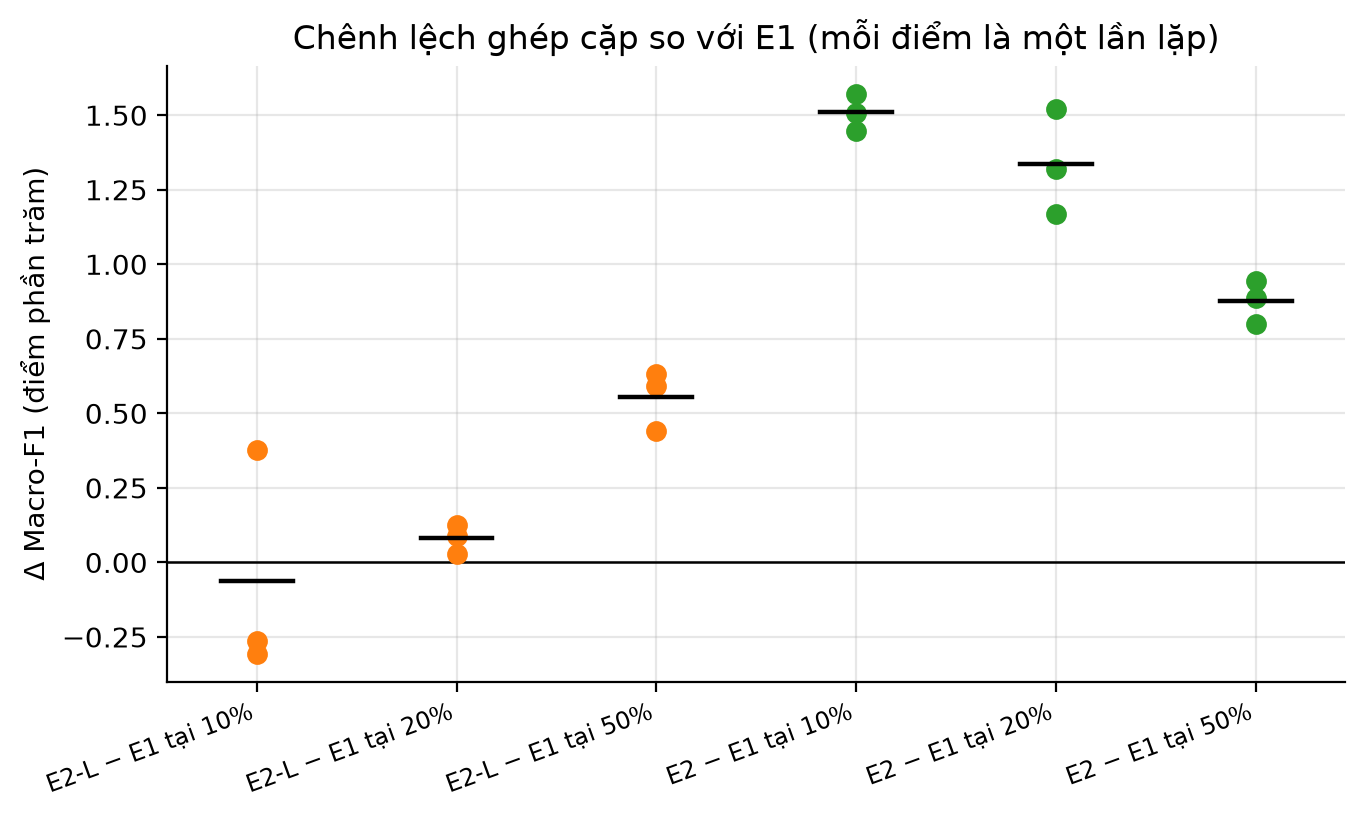
\includegraphics[width=0.95\textwidth]{../results/figures/fig03_paired_delta.png}
  \caption{Chênh lệch ghép cặp $\Delta_s$ so với \cfg{E1} ở cùng mức nhãn, tính bằng điểm phần
  trăm Macro-F1 trên $\Dtest$. Mỗi điểm là một lần lặp; vạch ngang là trung bình của ba lần
  lặp. Giá trị dương nghĩa là cấu hình đa nhiệm tốt hơn baseline.}
  \label{fig:paired-delta}
\end{figure}

\subsection{Hành vi hội tụ}
\label{sec:results-convergence}

Vì bảng kết quả chính không dùng Early Stopping, cần kiểm tra xem việc chạy đủ 100 epoch có dẫn
tới quá khớp lâu dài trên validation hay không. \tabref{tab:convergence} trình bày thời điểm đạt
checkpoint tốt nhất và mức suy giảm về cuối quá trình.

% Sinh tự động — scripts/make_report_data.py
\begin{table}[htbp]
  \centering
  \scriptsize
  \setlength{\tabcolsep}{4pt}
  \begin{tabular}{@{}l c c c r@{}}
    \toprule
    \makecell[l]{Cấu hình} & \makecell{Epoch\\tốt nhất} & \makecell{Macro-F1 val\\tại epoch tốt nhất} & \makecell{Macro-F1 val\\tại epoch cuối} & \makecell[r]{Khoảng\\cách} \\
    \midrule
    \cfg{E1} & 90,8 & 0,9521 & 0,9507 & +0,0014 \\
    \cfg{E2-L} & 85,3 & 0,9542 & 0,9524 & +0,0018 \\
    \cfg{E2} & 85,0 & 0,9644 & 0,9631 & +0,0014 \\
    \bottomrule
  \end{tabular}
  \caption{Hành vi hội tụ. \enquote{Khoảng cách} là Macro-F1 validation tại epoch tốt nhất trừ giá trị tại epoch cuối; giá trị dương nghĩa là mô hình bắt đầu suy giảm trên validation trước khi kết thúc 100 epoch. Vì không dùng Early Stopping, quá trình vẫn chạy tới epoch 100 như thiết kế.}
  \label{tab:convergence}
\end{table}

\subsection{Chỉ số từng lớp và phân tích lỗi}
\label{sec:results-perclass}

% Sinh tự động — scripts/make_report_data.py
\begin{table}[htbp]
  \centering
  \small
  \setlength{\tabcolsep}{6pt}
  \begin{tabular}{@{}l r r r r r@{}}
    \toprule
    & \multicolumn{2}{c}{Animal} & \multicolumn{2}{c}{Vehicle} & \\
    \cmidrule(lr){2-3}\cmidrule(lr){4-5}
    Cấu hình & Precision & Recall & Precision & Recall & F1 (Animal / Vehicle) \\
    \midrule
    \cfg{E1} & 0,9405 & 0,9517 & 0,9263 & 0,9096 & 0,9461 / 0,9178 \\
    \cfg{E2-L} & 0,9454 & 0,9447 & 0,9172 & 0,9181 & 0,9450 / 0,9176 \\
    \cfg{E2} & 0,9548 & 0,9608 & 0,9407 & 0,9318 & 0,9578 / 0,9362 \\
    \bottomrule
  \end{tabular}
  \caption{Precision, recall và F1 từng siêu lớp tại mức 10\,\% nhãn (trung bình ba lần lặp). Vì tỷ lệ Animal/Vehicle là 60/40, Accuracy đơn lẻ không phản ánh đầy đủ chất lượng của từng lớp.}
  \label{tab:per-class}
\end{table}

% Sinh tự động — scripts/make_report_data.py
\begin{table}[htbp]
  \centering
  \small
  \setlength{\tabcolsep}{6pt}
  \begin{tabular}{@{}l r r r r r@{}}
    \toprule
    & \multicolumn{2}{c}{Animal} & \multicolumn{2}{c}{Vehicle} & \\
    \cmidrule(lr){2-3}\cmidrule(lr){4-5}
    Cấu hình & Precision & Recall & Precision & Recall & F1 (Animal / Vehicle) \\
    \midrule
    \cfg{E1} & 0,9735 & 0,9769 & 0,9652 & 0,9602 & 0,9752 / 0,9627 \\
    \cfg{E2-L} & 0,9819 & 0,9772 & 0,9660 & 0,9730 & 0,9795 / 0,9695 \\
    \cfg{E2} & 0,9838 & 0,9805 & 0,9709 & 0,9758 & 0,9821 / 0,9733 \\
    \bottomrule
  \end{tabular}
  \caption{Precision, recall và F1 từng siêu lớp tại mức 50\,\% nhãn (trung bình ba lần lặp). Vì tỷ lệ Animal/Vehicle là 60/40, Accuracy đơn lẻ không phản ánh đầy đủ chất lượng của từng lớp.}
  \label{tab:per-class-50}
\end{table}

\begin{figure}[htbp]
  \centering
  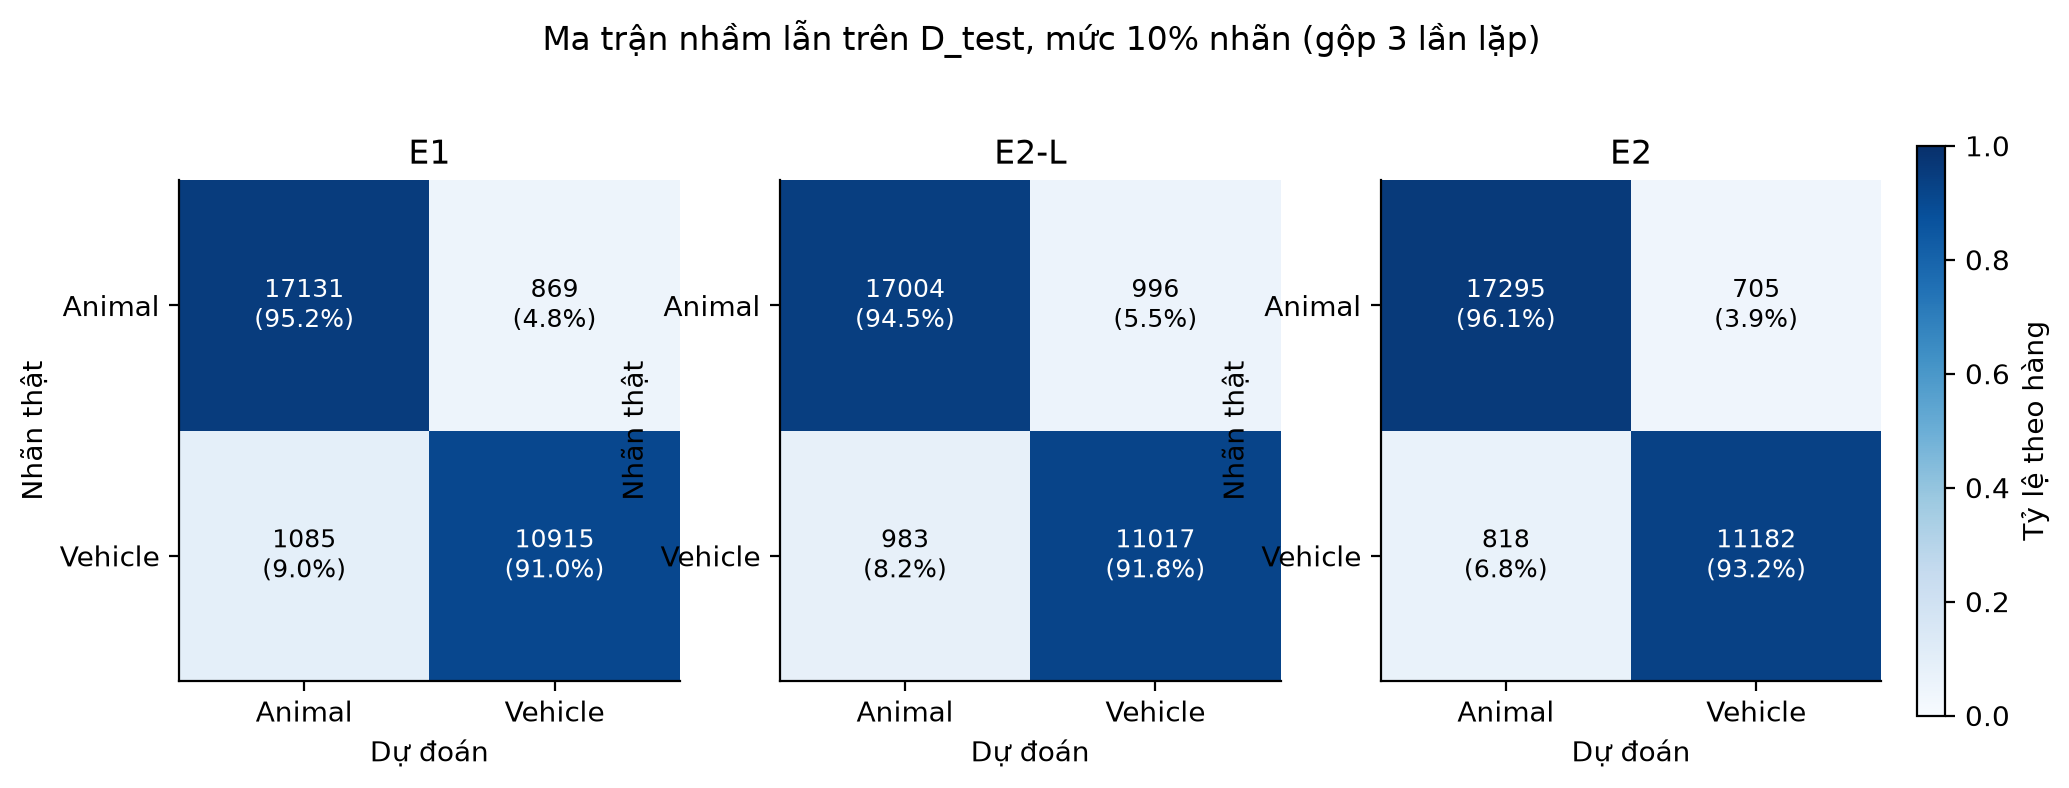
\includegraphics[width=\textwidth]{../results/figures/fig04_confusion_L10.png}
  \caption{Ma trận nhầm lẫn trên $\Dtest$ tại mức $10\,\%$ nhãn, gộp ba lần lặp (tổng 30.000
  dự đoán cho mỗi cấu hình). Ô ghi số lượng tuyệt đối và tỷ lệ theo hàng. Ma trận cho thấy
  phần lớn sai số tập trung ở lớp Vehicle bị dự đoán thành Animal.}
  \label{fig:confusion}
\end{figure}

\subsection{Chi phí huấn luyện và suy luận}
\label{sec:results-cost}

% Sinh tự động — scripts/make_report_data.py
\begin{table}[htbp]
  \centering
  \small
  \begin{tabular}{@{}l r r r@{}}
    \toprule
    Cấu hình & 10\,\% (giây/lượt) & 20\,\% (giây/lượt) & 50\,\% (giây/lượt) \\
    \midrule
    \cfg{E1} & 344,1 & 557,9 & 1.165,4 \\
    \cfg{E2-L} & 575,5 & 1.026,8 & 2.322,4 \\
    \cfg{E2} & 578,8 & 1.013,9 & 2.322,3 \\
    \bottomrule
  \end{tabular}
  \caption{Thời gian huấn luyện trung bình cho một lượt chạy 100 epoch. \cfg{E2-L} và \cfg{E2} xử lý thêm minibatch cho nhiệm vụ xoay ở mỗi bước cập nhật, nên chi phí học cao hơn \cfg{E1} một cách có hệ thống.}
  \label{tab:training-cost}
\end{table}

% Sinh tự động — scripts/make_report_data.py
\begin{table}[htbp]
  \centering
  \small
  \begin{tabular}{@{}l r@{}}
    \toprule
    Thành phần & Giá trị \\
    \midrule
    Tham số encoder $\enc$ & 11.168.832 \\
    Tham số Superclass Head & 1.026 \\
    Tham số Rotation Head & 2.052 \\
    Tổng tham số khi suy luận & \RParamInference \\
    Tổng tham số khi huấn luyện & \RParamTraining \\
    Dung lượng FP32 của mô hình suy luận & \RParamInferenceMiB{} MiB \\
    Dung lượng tệp trọng số suy luận đo được & \RParamInferenceFileMiB{} MiB \\
    \bottomrule
  \end{tabular}
  \caption{Chi phí tham số của mô hình tại cấu hình \secref{sec:arch}. Rotation Head chỉ tồn tại trong giai đoạn huấn luyện; khi suy luận chỉ cần encoder và Superclass Head. Dung lượng tệp được đo bằng cách lưu riêng trọng số suy luận, không gộp optimizer state.}
  \label{tab:inference-cost}
\end{table}

\paragraph{Vì sao \cfg{E2} đắt hơn \cfg{E2-L} — và vì sao khoảng cách đó thu hẹp theo mức nhãn.}
\tabref{tab:rotation-data-cost} đo riêng chi phí \emph{dựng view} của nhánh phụ. Ở mức
$10\,\%$ nhãn, nguồn $\Dtrain$ gấp $10$ lần nguồn $\DL$ về số view mỗi epoch; ở mức $50\,\%$
nhãn, tỷ lệ này chỉ còn $2$ lần. Đây là lý do định lượng cho việc \cfg{E2} đắt hơn \cfg{E2-L}
rõ rệt khi ít nhãn.

% Sinh tự động — scripts/make_report_data.py
\begin{table}[htbp]
  \centering
  \small
  \setlength{\tabcolsep}{6pt}
  \begin{tabular}{@{}r r r r r@{}}
    \toprule
    Mức nhãn & $|\DL|$ (view) & $|\Dtrain|$ (view) & Giây/epoch khi nguồn $= \DL$ & Giây/epoch khi nguồn $= \Dtrain$ \\
    \midrule
    10\,\% & 4.500 & 45.000 & 1,2 & 13,2 \\
    20\,\% & 9.000 & 45.000 & 2,7 & 13,7 \\
    50\,\% & 22.500 & 45.000 & 6,8 & 13,6 \\
    \bottomrule
  \end{tabular}
  \caption{Chi phí \emph{dựng view} cho nhánh xoay, đo riêng trên CPU, không gồm forward/backward. Bảng đo theo GIẢ ĐỊNH nhánh phụ duyệt hết tập nguồn mỗi epoch; trong mã nguồn thì $B_R$ được cắt về đúng $b_L$, nên số view \emph{thực dùng} mỗi epoch bằng $|\DL|$ ở cả \cfg{E2-L} và \cfg{E2}. Vì vậy chi phí dựng view thực tế của hai cấu hình gần như bằng nhau, và tỷ lệ nêu trên là chi phí của kịch bản giả định.}
  \label{tab:rotation-data-cost}
\end{table}

% Sinh tự động — scripts/make_report_data.py
\begin{table}[htbp]
  \centering
  \small
  \begin{tabular}{@{}l r r r@{}}
    \toprule
    Điều kiện đo & Mean (ms/ảnh) & Median (ms/ảnh) & p95 (ms/ảnh) \\
    \midrule
    CPU (4 luồng), FP32 & \RLatMeanCpu & \RLatMedianCpu & \RLatPNinetyFiveCpu \\
    GPU (RTX 5070 Laptop), FP32 & \RLatMeanGpu & \RLatMedianGpu & \RLatPNinetyFiveGpu \\
    \bottomrule
  \end{tabular}
  \caption{Độ trễ suy luận với batch $=1$, tensor $1 \times 3 \times 32 \times 32$, FP32, \code{model.eval()} và \code{torch.inference\_mode()}. Mỗi điều kiện khởi động 50 lượt rồi đo 1.000 lượt, lặp ba phiên. Cách tổng hợp ba phiên KHÔNG giống nhau: \emph{mean} và \emph{p95} là trung bình cộng của ba phiên, còn \emph{median} là trung vị của ba trung vị phiên (xem \code{src/m8/benchmark.py}). Phép đo chỉ tính thời gian tính toán của mô hình, không gồm đọc ảnh và tiền xử lý.}
  \label{tab:latency}
\end{table}

\paragraph{Đọc các số liệu chi phí.}
Độ trễ trung bình \RLatMeanCpu{}~ms/ảnh trên CPU (ghim \RLatThreads{} luồng) và
\RLatMeanGpu{}~ms/ảnh trên \REnvGpu{} ở chế độ đo đã đồng bộ CUDA. Con số p95 trên GPU
(\RLatPNinetyFiveGpu{}~ms) cao hơn trung vị (\RLatMedianGpu{}~ms) cho thấy phân bố thời gian không đối
xứng: một số lượt đo bị chi phối bởi chi phí phát lệnh và đồng bộ chứ không phải bởi phép tính
thực sự của mạng trên tensor nhỏ $1 \times 3 \times 32 \times 32$. Thời gian đọc ảnh và tiền xử
lý trên CPU được đo riêng và có giá trị \RPreprocessMs{}~ms/ảnh, tức cùng bậc độ lớn với thời
gian suy luận GPU; đây là yếu tố thường bị bỏ qua khi chỉ báo cáo \enquote{độ trễ mô hình}.

\paragraph{So sánh chi phí học giữa ba cấu hình.}
\tabref{tab:training-cost} cho thấy \cfg{E1} rẻ nhất, \cfg{E2-L} và \cfg{E2} đắt hơn do phải
xử lý thêm một minibatch ở mỗi bước cập nhật. Cần lưu ý rằng mức tăng này không tỷ lệ với số
epoch (cả ba cấu hình đều 100 epoch) mà tỷ lệ với số lượt ảnh được xử lý.
